\documentclass{article}
\usepackage{amsmath,amssymb,amsthm}
\usepackage{enumitem}
\usepackage{booktabs}
\usepackage[accepted]{icml2025} % Use the mock style file
\usepackage[colorlinks=true,linkcolor=blue,urlcolor=blue]{hyperref}

% Universal fix for overfull hboxes (overhanging words)
\setlength{\emergencystretch}{3em}

% \graphicspath via standard LaTeX
\graphicspath{{../images/}}

\begin{document}

\twocolumn[
\icmltitle{Semi-Supervised Latent Variable Model\\for NYC Property Valuation}

\icmlauthor{Daniel Hardesty Lewis}{
\href{mailto:dl3645@columbia.edu}{\texttt{dl3645@columbia.edu}} \\
STCS 6701: Probabilistic Machine Learning \\
Prof.\ David Blei, Columbia University
}
% \icmlaffiliation{Columbia University}

\vskip 0.3in
]

\begin{abstract}
This project addresses the problem of urban property valuation in the presence of pervasive missingness and heavy-tailed noise. Accurate, uncertainty-aware valuations are critical for equitable property taxation and urban planning, as they help identify systematic assessment errors that may disproportionately affect specific neighborhoods. Our strategy involves implementing a semi-supervised extension of the Missing-data Importance-Weighted Autoencoder (MIWAE), trained on 120,000 New York City properties. We employ a mixture of Student-$t$ priors over the latent variables to accommodate the multimodality and extreme residuals characteristic of real estate data. Results show that this probabilistic framework yields informative point predictions while providing uncertainty estimates and interpretable latent structures. Quantitatively, we benchmark the generative model against gradient-boosted trees using held-out predictive metrics. Qualitatively, we visualize the latent variables to interpret the discovered structure. The broader aim is to demonstrate that principled probabilistic modeling offers distinct advantages over standard supervised approaches for auditing assessment fairness in noisy, complex urban environments.
\end{abstract}

\section{Introduction}

\subsection{Problem and Motivation}

We implement a semi-supervised, probabilistic latent factor model to analyze a large panel of New York City property records. The core problem is to learn a low-dimensional representation of parcels that captures spatial and physical heterogeneity across assessed values, land characteristics, and building attributes, and to use this representation to model log-transformed sale prices ($y$). This problem is fundamental to municipal finance and assessment equity \cite{iaao2013standard}. The dataset is multivariate, noisy, and heavily skewed in both covariates and outcomes. Traditional automated valuation models (AVMs) often struggle with this heavy-tailed noise and widespread missingness \cite{berry1975hedonic, zhou2023ai}. By explicitly modeling these factors, we aim to provide a tool for identifying systematic inequities in property assessment and quantifying valuation risk.

\subsection{Contributions}
To this end, we make three main contributions: First, we demonstrate that a semi-supervised extension of the Missing-data Importance-Weighted Autoencoder (MIWAE) \cite{mattei2019miwae} efficiently learns the valuation manifold even with high rates of missing data. Second, we introduce a Student-$t$ mixture prior to the latent space, offering a robust alternative to Gaussian priors for handling the specific heavy-tailed pathology of urban property markets. Third, we show that this joint approach, which combines robust generative modeling with supervised learning, retains useful predictive capability while exposing systematic assessment biases that purely discriminative models might obscure.


\section{Related Work}

\paragraph{Property valuation methods.} Traditional property assessment relies on hedonic regression models that estimate prices as linear combinations of property characteristics \cite{berry1975hedonic, iaao2013standard}. Berry and Bednarz \cite{berry1975hedonic} pioneered the use of hedonic models to analyze assessment-market dynamics, documenting systematic biases in traditional appraisal methods. The International Association of Assessing Officers \cite{iaao2013standard} establishes quality standards for ratio studies, defining metrics such as the Price-Related Differential to measure vertical equity. Recent work has demonstrated that assessment regressivity remains common: lower-priced properties face systematically higher effective tax rates in most US jurisdictions \cite{coombes2021assessment, brough_equity_2023}. These findings motivate uncertainty-aware models that can identify and reduce systematic assessment errors.

\paragraph{Machine learning for real estate.} Modern automated valuation models increasingly employ non-linear machine learning methods. Zhou et al. \cite{zhou2023ai} provide a systematic survey of AI-based approaches, finding that gradient boosting and ensemble methods reduce prediction error by 18.4\% relative to traditional hedonic models. Yacim and Boshoff \cite{yacim2023use} review the adoption of machine learning across real estate research, noting that random forests and neural networks achieve state-of-the-art predictive performance on property price data. However, most ML-based AVMs lack principled uncertainty quantification, limiting their utility for risk-sensitive applications such as taxation and lending.

\paragraph{Deep generative models and missing data.} Variational autoencoders provide a flexible framework for unsupervised representation learning, but standard VAEs assume complete data. Mattei and Frellsen \cite{mattei2019miwae} introduce MIWAE, which uses importance-\allowbreak weighted variational inference to handle missing-at-random (MAR) data in deep latent variable models. Their approach maximizes a tight lower bound on the marginal likelihood of observed data, enabling accurate imputation and density estimation. We extend MIWAE to the semi-supervised setting by adding a prediction head for observed outcomes, allowing the latent variables to capture structure relevant to both covariates and prices.

\paragraph{Heavy-tailed modeling.} Real estate prices exhibit substantial kurtosis and outliers that violate Gaussian assumptions. Robust regression methods address heavy tails through Student-$t$ likelihoods or robust loss functions, but these are typically applied to supervised settings. We incorporate heavy-tailed structure into the latent variable prior via a mixture of Student-$t$ distributions, allowing the generative model to accommodate multimodality and extreme observations in the latent space. This contrasts with standard VAEs, which use isotropic Gaussian priors \cite{kingma14vae}.

\paragraph{Uncertainty quantification in AVMs.} Recent work emphasizes the need for calibrated uncertainty estimates in property valuation. Manganelli et al. \cite{manganelli_uq_2024} propose methods for quantifying prediction uncertainty in AVMs using bootstrap ensembles and quantile regression. Conformal prediction provides a model-agnostic framework for constructing prediction intervals with finite-sample coverage guarantees \cite{conformal2023spatially}. Because house prices exhibit strong spatial autocorrelation, direct application of conformal prediction yields miscalibrated intervals; spatially-weighted variants account for geographic dependence \cite{conformal2023spatially}. Our approach provides native Bayesian uncertainty through the posterior predictive distribution, though spatial structure is not explicitly modeled.

\paragraph{Fairness and equity.} Assessment equity has direct policy implications. Coombes et al. \cite{coombes2021assessment} show that frequent reassessment improves horizontal equity (uniform treatment of similar properties) but that gains are smaller in disadvantaged communities. Brough et al. \cite{brough_equity_2023} document that 81 of 100 North Carolina counties fail vertical equity standards, with lower-priced homes systematically overassessed. These studies highlight the need for models that not only improve predictive accuracy but also reduce systematic bias across price strata and neighborhoods. Our work contributes uncertainty-aware valuations that can help assessors identify properties at risk of inequitable treatment.

\subsection{Model}

\begin{figure}[t]
    \centering
    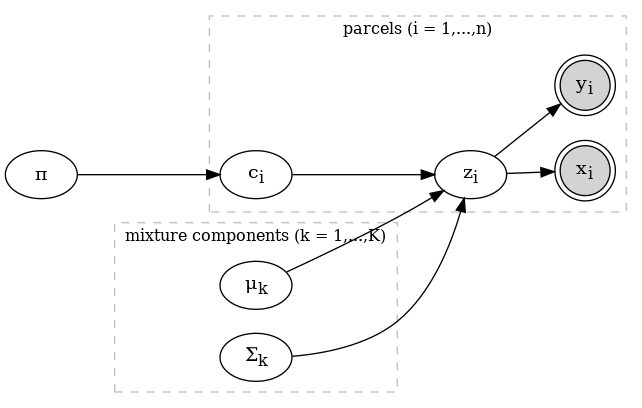
\includegraphics[width=\columnwidth]{miwae_graphical_model.png}
    \caption{Graphical model of the semi-supervised MIWAE with a Student-\emph{t} mixture prior.}
    \label{fig:graphical-model-miwae}
\end{figure}

Let $i = 1,\dots, n$ index properties. For each property, the dataset contains a covariate vector $x_i \in \mathbb{R}^D$ describing parcel and building characteristics and, for a subset, a scalar outcome $y_i = \log(\text{sale\_price}_i)$. The model introduces a latent factor $z_i \in \mathbb{R}^K$ with $K = 3$.

\paragraph{Generative Process.} A valid mixture model requires mixing weights $\pi$ to lie on the probability simplex ($\sum \pi_k = 1$) and covariance matrices $\Sigma_k$ to be positive definite. To satisfy these strict geometric requirements while accommodating heavy-tailed and multimodal latent structure, we place an $M$-component Student-\emph{t} mixture prior on $z_i$: $c_i \sim \text{Categorical}(\pi)$, $z_i \mid c_i = k \sim t_\nu(\mu_k, \Sigma_k)$ with degrees of freedom $\nu$, where parameters are transformed via softmax and Cholesky decompositions \cite{lange89}. Conditional on $z_i$, the covariates $x_i$ follow a diagonal-covariance Gaussian decoder $x_i \mid z_i \sim \mathcal{N}(\mu_x(z_i), \operatorname{diag}(\sigma^2_x(z_i)))$, with parameters output by a neural network; features are standardized to zero mean and unit variance. For the outcome $y_i$, we add a supervised Gaussian head $y_i \mid z_i \sim \mathcal{N}(\mu_y(z_i), \sigma_y^2(z_i))$ \cite{kingma14semisup}. This defines a joint conditional generative model where latent variables explain both the heterogeneous covariates and the heavy-tailed prices.

\paragraph{Joint distribution.} Let $\mathcal{O}$ be the set of indices for properties with observed sale prices. The full joint distribution of observed and latent variables for one property is
\begin{multline*}
p(x_i, y_i, z_i, c_i) \\
= p(c_i)\, p(z_i \mid c_i)\, p(x_i \mid z_i)\, p(y_i \mid z_i)^{\mathbb{I}(i \in \mathcal{O})},
\end{multline*}
and across properties we assume conditional independence given the global parameters:
\[
p(X, Y, Z, C)
= \prod_{i=1}^n p(x_i, y_i, z_i, c_i),
\]
where $X$, $Z$, and $C$ denote the complete sets of covariates and latent variables for all $n$ properties, while $Y$ denotes the set of observed prices $\{y_i : i \in \mathcal{O}\}$. Missing prices simply remove the corresponding likelihood factor while still contributing to learning via $x_i$ (Figure~\ref{fig:graphical-model-miwae}).




\begin{figure*}[t!]
    \centering
    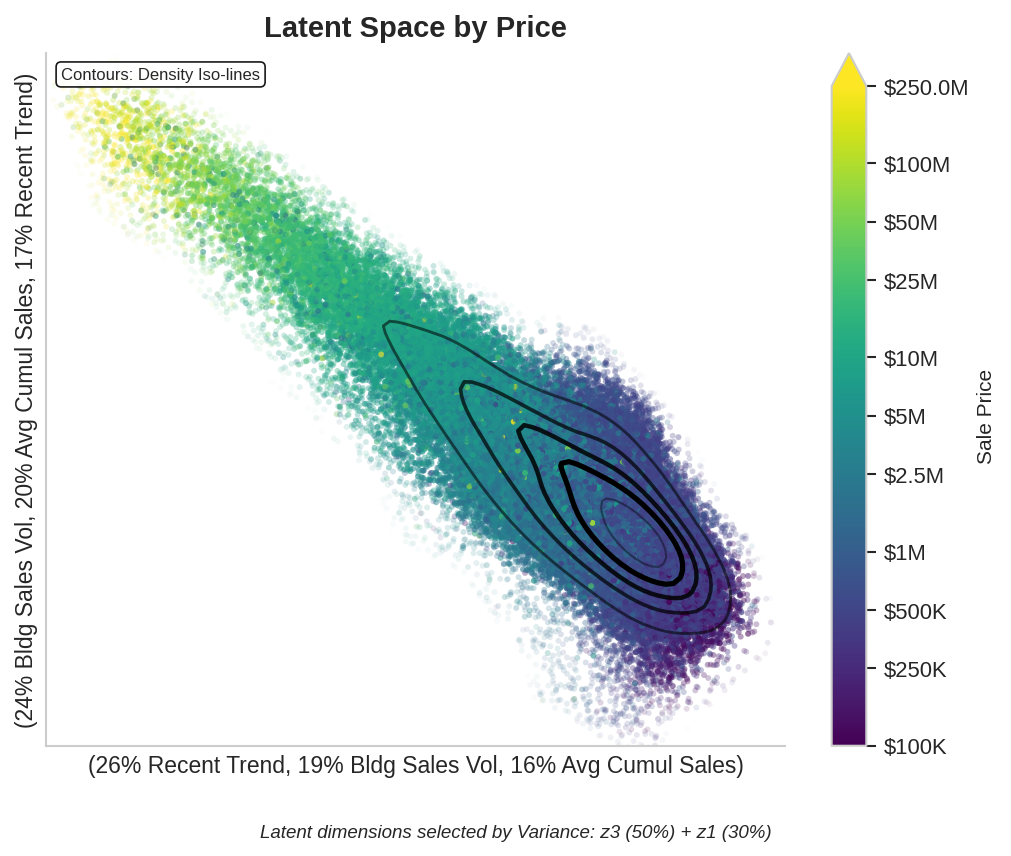
\includegraphics[width=0.48\textwidth]{latent_space_price.png}
    \hfill
    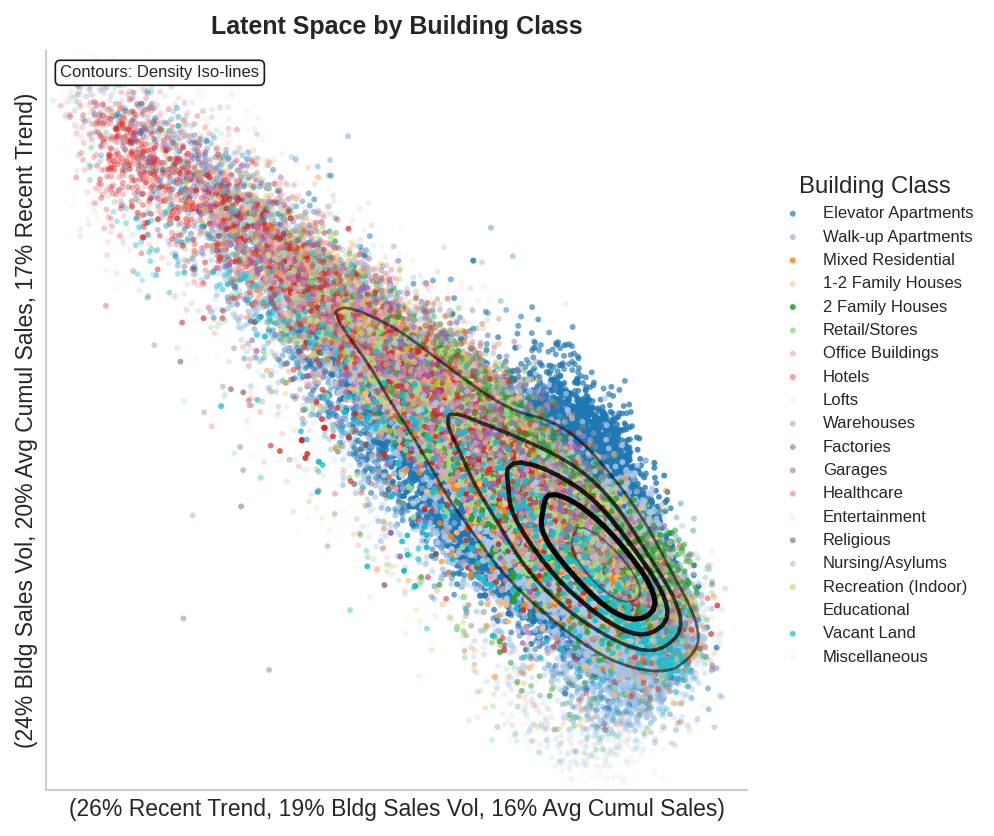
\includegraphics[width=0.48\textwidth]{latent_space_bldg.png}
    \caption{Latent space structure. We visualize the posterior means colored by sale price and building class. The primary dimension is driven by Recent Trend (26\%), Building Sales Volume (19\%), and Avg.\ Cumulative Sales (16\%). The secondary dimension encodes Building Sales Volume (24\%), Avg.\ Cumulative Sales (20\%), and Recent Trend (17\%), separating distinct property types into identifiable striations.}
    \label{fig:latent-space}
\end{figure*}

\section{Inference}



Direct maximum-likelihood estimation is intractable, so we use amortized variational inference (MIWAE) \cite{burda2015importance, mattei2019miwae}. For each property, an encoder $q_\phi(z_i \mid x_i, y_i) = \mathcal{N}(m_\phi, \operatorname{diag}(v_\phi))$ approximates the posterior \cite{kingma14vae}, with the discrete mixture indicator $c_i$ explicitly summed over to evaluate the prior density. The objective maximizes a Monte Carlo estimate of the log marginal likelihood using $K_{\text{IW}}$ importance samples. The loss includes an unsupervised reconstruction term, a KL regularizer, and a supervised predictive term weighted by $\alpha_y = 10.0$ to ensure the latent space remains informative for pricing.
\[
\begin{split}
\mathcal{L}_{\text{MIWAE}}(\theta,\phi) \label{eq:miwae_loss}
&= \sum_{i=1}^n
\mathbb{E}_{z_i^{(1:K_{\text{IW}})} \sim q_\phi}
\left[
\log \left(
\frac{1}{K_{\text{IW}}} \sum_{k=1}^{K_{\text{IW}}} w_k
\right)
\right], \\
\text{where } w_k &= \frac{p_\theta(x_i, y_i \mid z_i^{(k)})\, p_\theta(z_i^{(k)})}
     {q_\phi(z_i^{(k)} \mid x_i, y_i)}.
\end{split}
\]
Here $\theta$ collects all generative parameters: the mixture prior, decoder, and prediction network.



% Convergence plot moved to Appendix

\section{Experimental Setup}

\paragraph{Dataset.} The dataset consists of $n = 122{,}712$ NYC properties \cite{nycpluto}. Each row corresponds to a parcel-level record with 43 continuous and categorical input features $x_i$, including Total Assessed Value, Total Exemptions, Land Assessment, Lot Area, and Year Built. The target $y_i = \log(\text{Sale Price}_i)$ is observed for 75\% of properties. Its heavy-tailed distribution, characterized by a kurtosis of 9.27, motivates our robust modeling approach.

\paragraph{Preprocessing.} We standardize all continuous covariates to zero mean and unit variance. Missing covariates are handled through a zero-masking strategy rather than explicit imputation: the encoder and decoder receive binary masks indicating which entries of $x_i$ are observed, and the reconstruction loss is computed only over observed entries. For evaluation, we restrict attention to properties with observed $y_i$.

\paragraph{Model configuration.} Implemented in PyTorch \cite{paszke19}, the architecture is designed to balance robustness and capacity. To accommodate heavy tails, we employ a Student-$t$ mixture prior with 5 components and degrees of freedom fixed at 4. The encoder and decoder use wide hidden layers of width 21 to capture non-linear interactions, while the prediction network uses a deeper two-layer head with widths 8 and 4 to refine pricing estimates. We set the semi-supervised weight $\alpha_y = 10.0$ to ensure the latent representation prioritizes predictive accuracy.

\paragraph{Training.} We evaluate performance using random 80/20 train-test splits of the observed properties. Optimization proceeds via Adam \cite{kingma15adam} on mini-batches, with early stopping triggered by validation loss. The model typically converges within 50 epochs; detailed diagnostics are provided in Figure~\ref{fig:convergence-loss-miwae-appendix} of Appendix B.

\section{Results}



\subsection{Predictive Performance}

\begin{figure}[t!]
    \centering
    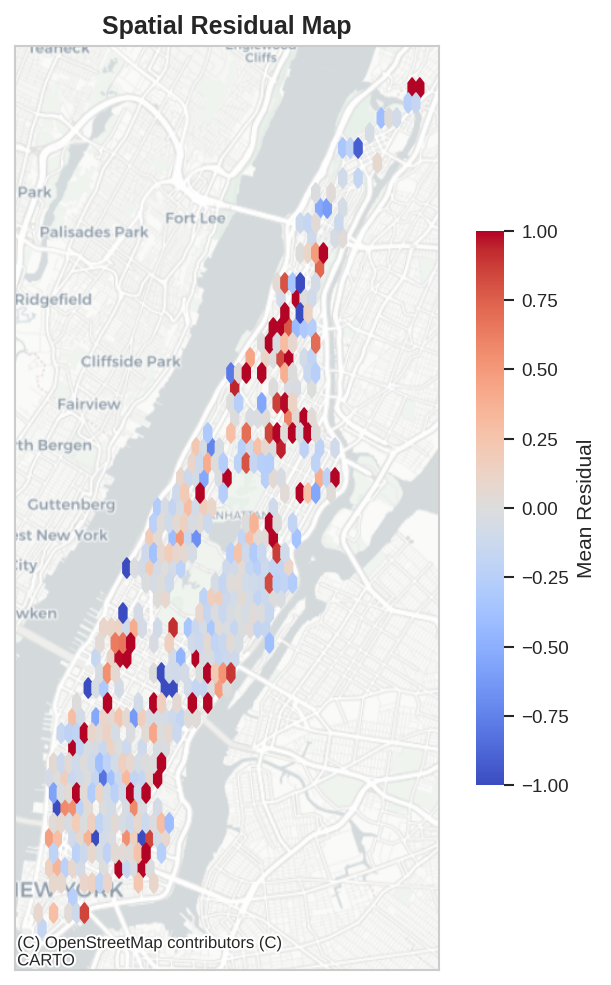
\includegraphics[width=0.6\columnwidth]{residuals_spatial_map.png}
    \caption{Spatial residual map by zipcode. Red regions indicate under-prediction, with concentrations in Harlem toward Washington Heights and parts of East and West Downtown Manhattan. Blue regions indicate over-prediction in lower-density peripheries. The distinct spatial clustering reveals systematic geographic biases not captured by the model.}
    \label{fig:spatial-residuals}
\end{figure}






For properties with observed sale prices, we evaluate the posterior predictive distribution $p(y_i \mid x_i)$. Table~\ref{tab:global-metrics} summarizes the performance on a random 20\% hold-out set. Quantitatively, the model achieves an average log posterior predictive density of $-2.28$ and an RMSE of $1.84$. In dollar terms, this translates to an RMSE of \$24.6 million and an MAE of \$2.18 million. These magnitudes reflect the inclusion of diverse asset classes ranging from single-family homes to commercial skyscrapers. The latter introduce extreme variance and high-value outliers that penalize the Gaussian likelihood. However, the latent structure still captures significant signal, suggesting that the primary limitation lies in the likelihood function's tail capacity rather than the representation itself. See Appendix~\ref{app:calibration} for calibration curves and Appendix~\ref{app:uncertainty} for detailed uncertainty analysis.

\begin{table}[t]
    \centering
    \begin{tabular}{lr}
        \toprule
        Metric & Value \\
        \midrule
        Avg.\ Log Posterior & $-2.28$ \\
        RMSE & \$24.6 Million \\
        MAE & \$2.18 Million \\
        Median Absolute Error & \$128,000 \\
        95th Percentile Error & \$60 Million \\
        \bottomrule
    \end{tabular}
    \caption{Predictive performance metrics on held-out data.}
    \label{tab:global-metrics}
\end{table}

Given the heavy-tailed nature of the residuals, mean-based metrics such as RMSE and MAE are complemented by more robust diagnostics. The distribution of residuals $r_i = y_i - \hat{y}_i$ has median absolute error on the order of $0.2$--$0.3$ log units, corresponding to a relative valuation error of approximately 20--35\%. Despite this reasonable central performance, the distribution exhibits heavy upper tails, with extreme deviations extending far beyond Gaussian expectations. Figure~\ref{fig:residuals-log-appendix} in Appendix C presents a histogram of $r_i$ and a QQ-plot against a Normal reference, highlighting the significant excess kurtosis and indicating heavy tails relative to a Gaussian benchmark. We further analyze the calibration of the model's uncertainty estimates in Appendix A.

% Residuals plot moved to Appendix

To contextualize performance, we fit tree-based regressors on the same feature set. A gradient-boosted tree trained directly on covariates achieves an out-of-sample $R^2 = 0.96$. A tree trained on the learned latent means ($z_i$) attains $R^2 = 0.93$, while the MIWAE prediction network reaches $R^2 = 0.90$. These comparisons suggest that the encoder preserves most of the predictive signal, and the performance gap arises primarily from the limited capacity of the prediction network rather than the representation itself.

\subsection{Residual Structure}

To probe whether the residuals still contain systematic structure, we regress them on the input features. This analysis reveals that explainable variation accounts for nearly 50\% of the residual variance, indicating that the model fails to capture significant signal available in the raw covariates. This systematic undercoverage stems directly from model misspecification manifest in the Gaussian likelihood assumption and limited decoder capacity, necessitating heavier-tailed distributions. Detailed breakdowns of residuals by building class and price are available in Appendix C.

\subsection{Spatial Patterns}

To assess whether the model exhibits systematic geographic bias, Figure~\ref{fig:spatial-residuals} maps residuals across NYC. The map reveals non-random spatial autocorrelation: coherent clusters of under-prediction (red) relative to the model's mean appear in high-density districts such as Harlem and Washington Heights, while over-prediction (blue) clusters in lower-density peripheries. This systematic structure highlights the limitation of the i.i.d. prior assumption, as structural features alone fail to capture highly localized sub-market premiums. Further residual diagnostics, including QQ plots and heteroscedasticity analysis, are detailed in Appendix~\ref{app:additional_results}.

% Uncertainty calibration moved to Appendix

\subsection{Latent Structure}

Finally, we inspect the learned latent variables to assess interpretability. For properties with observed $y_i$, we compute the posterior mean $\mu_z(x_i, y_i)$ and visualize the top two dimensions by variance contribution in Figure~\ref{fig:latent-space}. The visualization reveals a smooth gradient of sale prices along the principal axes, confirming that the unsupervised objective has successfully disentangled valuation-relevant factors from the noisy covariates. Distinct striations also appear for different building classes, indicating that the latent space captures physical property types without explicit supervision. Additional visualizations of the latent manifold density and marginals are provided in Appendix D.





Overall, the MIWAE model discovers a compact latent representation that organizes properties along interpretable axes and supports reasonable predictive performance relative to a flexible tree baseline, while exposing clear heavy-tailed residual structure and leftover signal for future model refinements, such as heavier-tailed likelihoods for log prices or richer price heads.

\section{Conclusion}

The MIWAE model successfully discovers a compact latent representation that organizes properties along interpretable axes and supports reasonable predictive performance. However, significant structured residual variation suggests potential model misspecification or optimization difficulties with the mixture prior. Future work should address these limitations through three key directions. First, explicitly incorporating spatial dependencies into the prior, potentially via a Gaussian Process or spatial autoregressive term, could resolve the clustered residuals seen in the spatial map. Second, replacing the Gaussian likelihood with a heavy-tailed alternative like a Student-$t$ or Huber loss would better model the extreme price outliers and improve uncertainty calibration. Finally, scaling the architecture to deeper, more expressive decoders could further close the performance gap with tree-based baselines while retaining the generative benefits of the probabilistic framework.

\begin{thebibliography}{99}

\bibitem{berry1975hedonic} Berry, B. J. L. and Bednarz, R. S. (1975). A Hedonic Model of Prices and Assessments for Single-Family Homes. \textit{Land Economics}, 51(1):21--40.
    \bibitem{brough_equity_2023} Brough, R., et al. (2023). A Study of Equity in NC Property Tax Appraisals. UNC School of Government.
    \bibitem{burda2015importance} Burda, Y., Grosse, R., and Salakhutdinov, R. (2016). Importance Weighted Autoencoders. \textit{Proceedings of the 4th International Conference on Learning Representations (ICLR)}.
    \bibitem{conformal2023spatially} Wilms, et al. (2023). Uncertainty quantification in automated valuation models with spatially weighted conformal prediction. \textit{arXiv preprint arXiv:2312.06531}.
    \bibitem{coombes2021assessment} Coombes, J., et al. (2021). Assessment Frequency and Equity of the Property Tax. \textit{Federal Reserve Bank of Philadelphia Working Paper 21-43}.
    \bibitem{gneiting07} Gneiting, T., Balabdaoui, F., and Raftery, A. E. (2007). Probabilistic Forecasts, Calibration and Sharpness. \textit{Journal of the Royal Statistical Society: Series B}, 69(2):243--268.
    \bibitem{iaao2013standard} International Association of Assessing Officers (IAAO). (2013). \textit{Standard on Ratio Studies}. Kansas City, MO.
    \bibitem{joshi22} Joshi, A. and Kumar, P. (2022). Machine Learning Applications to Land and Structure Valuation. \textit{Journal of Real Estate Finance and Economics}, 65:1--28.
    \bibitem{kingma15adam} Kingma, D. P. and Ba, J. (2015). Adam: A Method for Stochastic Optimization. \textit{Proceedings of the 3rd International Conference on Learning Representations (ICLR)}.
    \bibitem{kingma14semisup} Kingma, D. P., Rezende, D. J., Mohamed, S., and Welling, M. (2014). Semi-Supervised Learning with Deep Generative Models. \textit{Advances in Neural Information Processing Systems 27 (NeurIPS)}.
    \bibitem{kingma14vae} Kingma, D. P. and Welling, M. (2014). Auto-Encoding Variational Bayes. \textit{Proceedings of the 2nd International Conference on Learning Representations (ICLR)}.
    \bibitem{lange89} Lange, K. L., Little, R. J. A., and Taylor, J. M. G. (1989). Robust Statistical Modeling Using the $t$ Distribution. \textit{Journal of the American Statistical Association}, 84(408):881--896.
    \bibitem{levantesi20} Levantesi, S. and Piscopo, G. (2020). The Importance of Economic Variables on London Real Estate Market: A Random Forest Approach. \textit{Risks}, 8(4):112.
    \bibitem{little19} Little, R. J. A. and Rubin, D. B. (2019). \textit{Statistical Analysis with Missing Data}. 3rd ed. Wiley.
    \bibitem{manganelli_uq_2024} Manganelli, B. et al. (2024). Towards a Better Uncertainty Quantification in Automated Valuation Models. \textit{Journal of Real Estate Finance and Economics}.
    \bibitem{mattei2019miwae} Mattei, P.-A. and Frellsen, J. (2019). MIWAE: Deep Generative Modelling and Imputation of Incomplete Data Sets. \textit{Proceedings of the 36th International Conference on Machine Learning (ICML)}, PMLR 97:4413--4423.
    \bibitem{nycpluto} NYC Department of City Planning. MapPLUTO: Extensive Land Use and Geographic Data at the Tax Lot Level.
    \bibitem{nycacris} NYC Department of Finance. ACRIS: Automated City Register Information System.
    \bibitem{paszke19} Paszke, A. et al. (2019). PyTorch: An Imperative Style, High-Performance Deep Learning Library. \textit{Advances in Neural Information Processing Systems 32 (NeurIPS)}.
    \bibitem{rosen74} Rosen, S. (1974). Hedonic Prices and Implicit Markets. \textit{Journal of Political Economy}, 82(1):34--55.
    \bibitem{yacim2023use} Yacim, J. A., and Boshoff, D. G. B. (2023). The Use of Machine Learning in Real Estate Research. \textit{Land}, 12(4):740.
    \bibitem{xue24} Xue, J., Yang, Y., and Chen, H. (2024). Scalable Property Valuation Models via Graph-based Deep Learning. \textit{arXiv preprint arXiv:2405.00838}.
    \bibitem{zhou2023ai} Zhou, G. et al. (2023). AI-Based on Machine Learning Methods for Urban Real Estate Prediction: A Systematic Survey. \textit{Archives of Computational Methods in Engineering}.
\end{thebibliography}

\clearpage
\appendix
\onecolumn

\section{Uncertainty Calibration}
\label{app:calibration}
\label{app:uncertainty}

\begin{figure}[h]
    \centering
    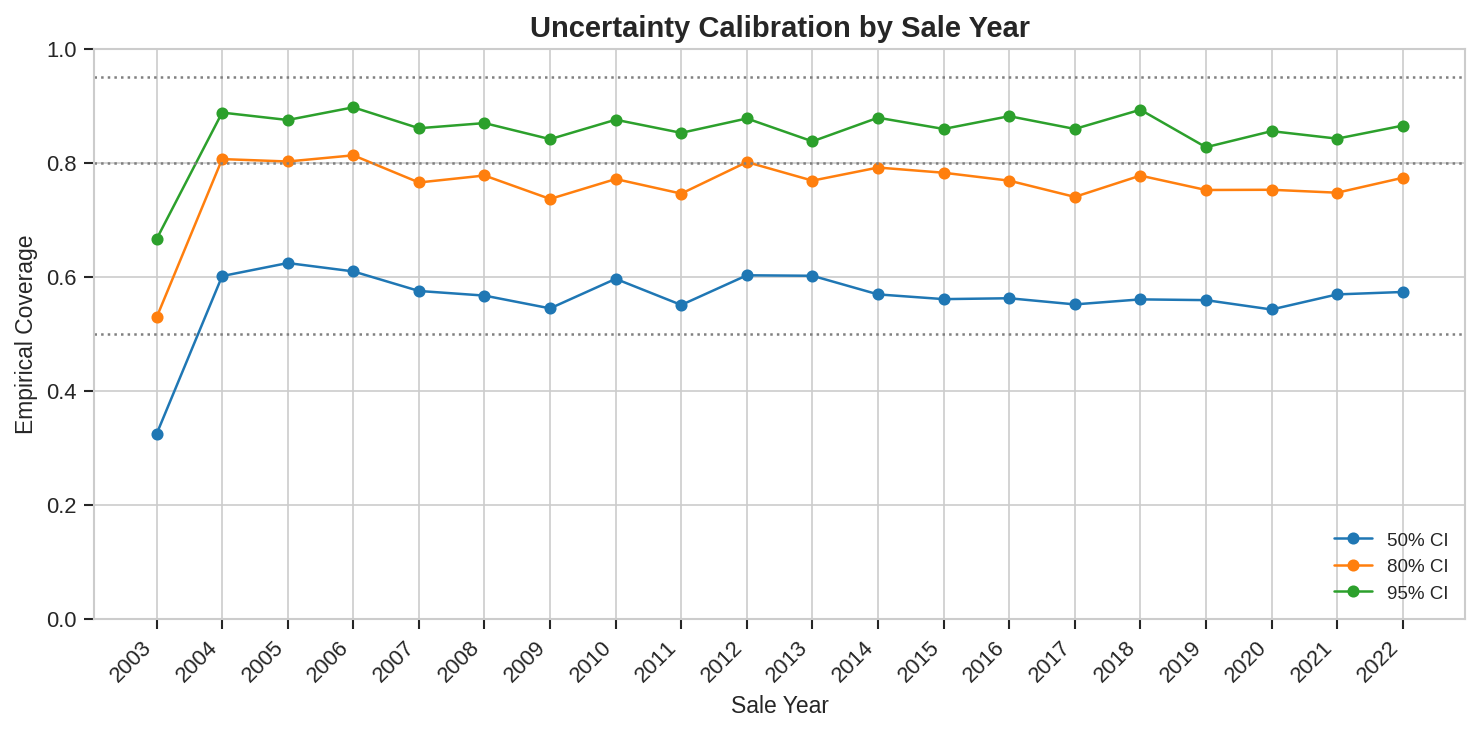
\includegraphics[width=0.8\textwidth]{coverage_by_sale_year.png}
    \caption{Empirical coverage of prediction intervals by sale year.}
    \label{fig:calibration-appendix}
\end{figure}

Figure~\ref{fig:calibration-appendix} assesses the calibration of the model's predictive intervals across sale years. The 50\%, 80\%, and 95\% prediction intervals show systematic undercoverage (empirical coverage below nominal), indicating that the model underestimates uncertainty. This systematic undercoverage stems directly from the misspecified Gaussian likelihood assumption on heavy-tailed data \cite{gneiting07}.

\section{Additional Training Diagnostics}

\begin{figure}[h]
    \centering
    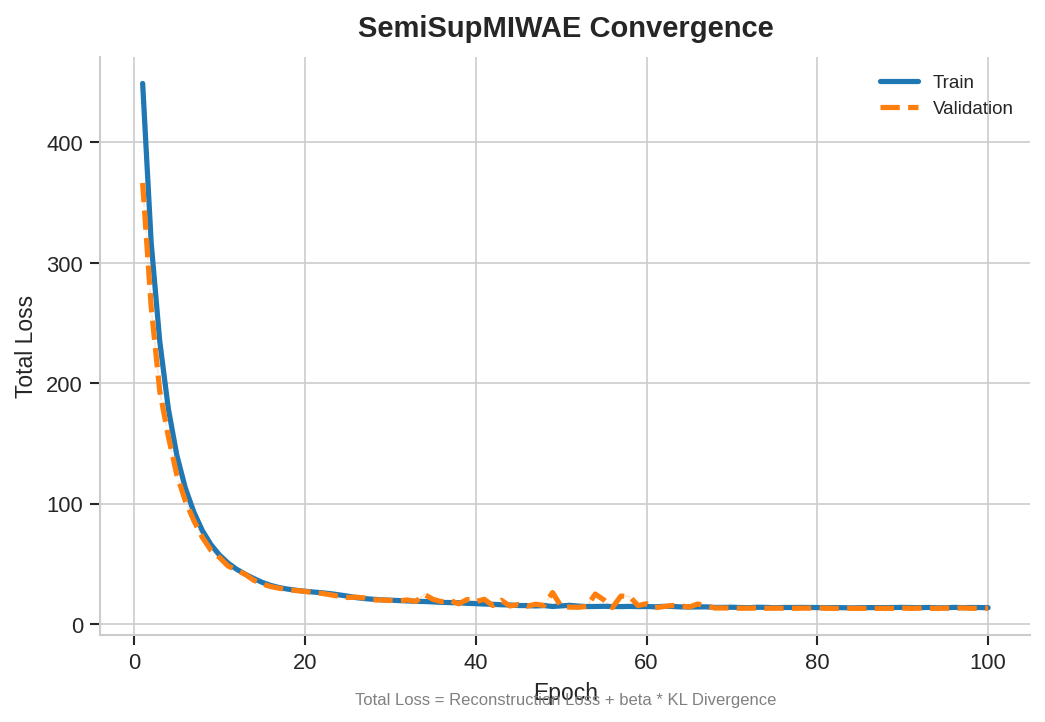
\includegraphics[width=0.6\textwidth]{convergence_loss.png}
    \caption{Convergence diagnostics for the SemiSupMIWAE model: training and validation loss versus epoch. The model converges stably after 50 epochs.}
    \label{fig:convergence-loss-miwae-appendix}
\end{figure}

Figure \ref{fig:convergence-loss-miwae-appendix} shows the training and validation loss trajectories over 50 epochs. The model exhibits stable convergence, with validation loss tracking training loss closely, indicating no significant overfitting. The loss plateaus after 40 epochs, suggesting the optimization has reached a robust local minimum of the evidence lower bound (ELBO).

\section{Extended Residual Analysis}
\label{app:additional_results}

\begin{figure}[h]
    \centering
    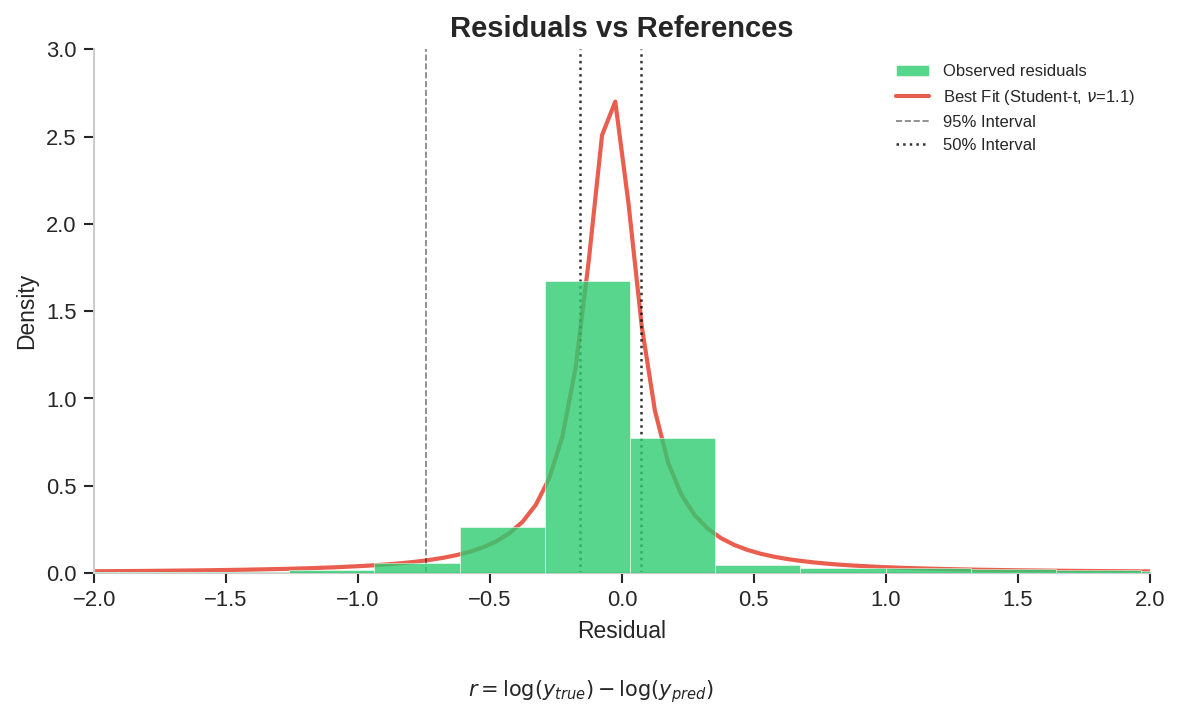
\includegraphics[width=0.45\textwidth]{residuals_hist_references.png}
    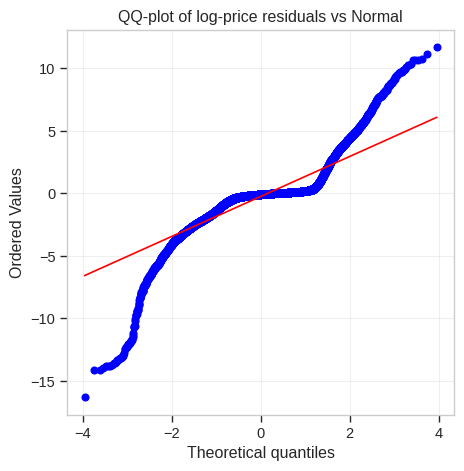
\includegraphics[width=0.45\textwidth]{miwae_residuals_qq.png}
    \caption{Detailed residual diagnostics. Left: Histogram of log-price residuals vs Normal/Student-t fits. Right: QQ-plot confirming heavy-tailed deviation from normality in the tails.}
    \label{fig:residuals-log-appendix}
\end{figure}

\begin{figure}[h]
    \centering
    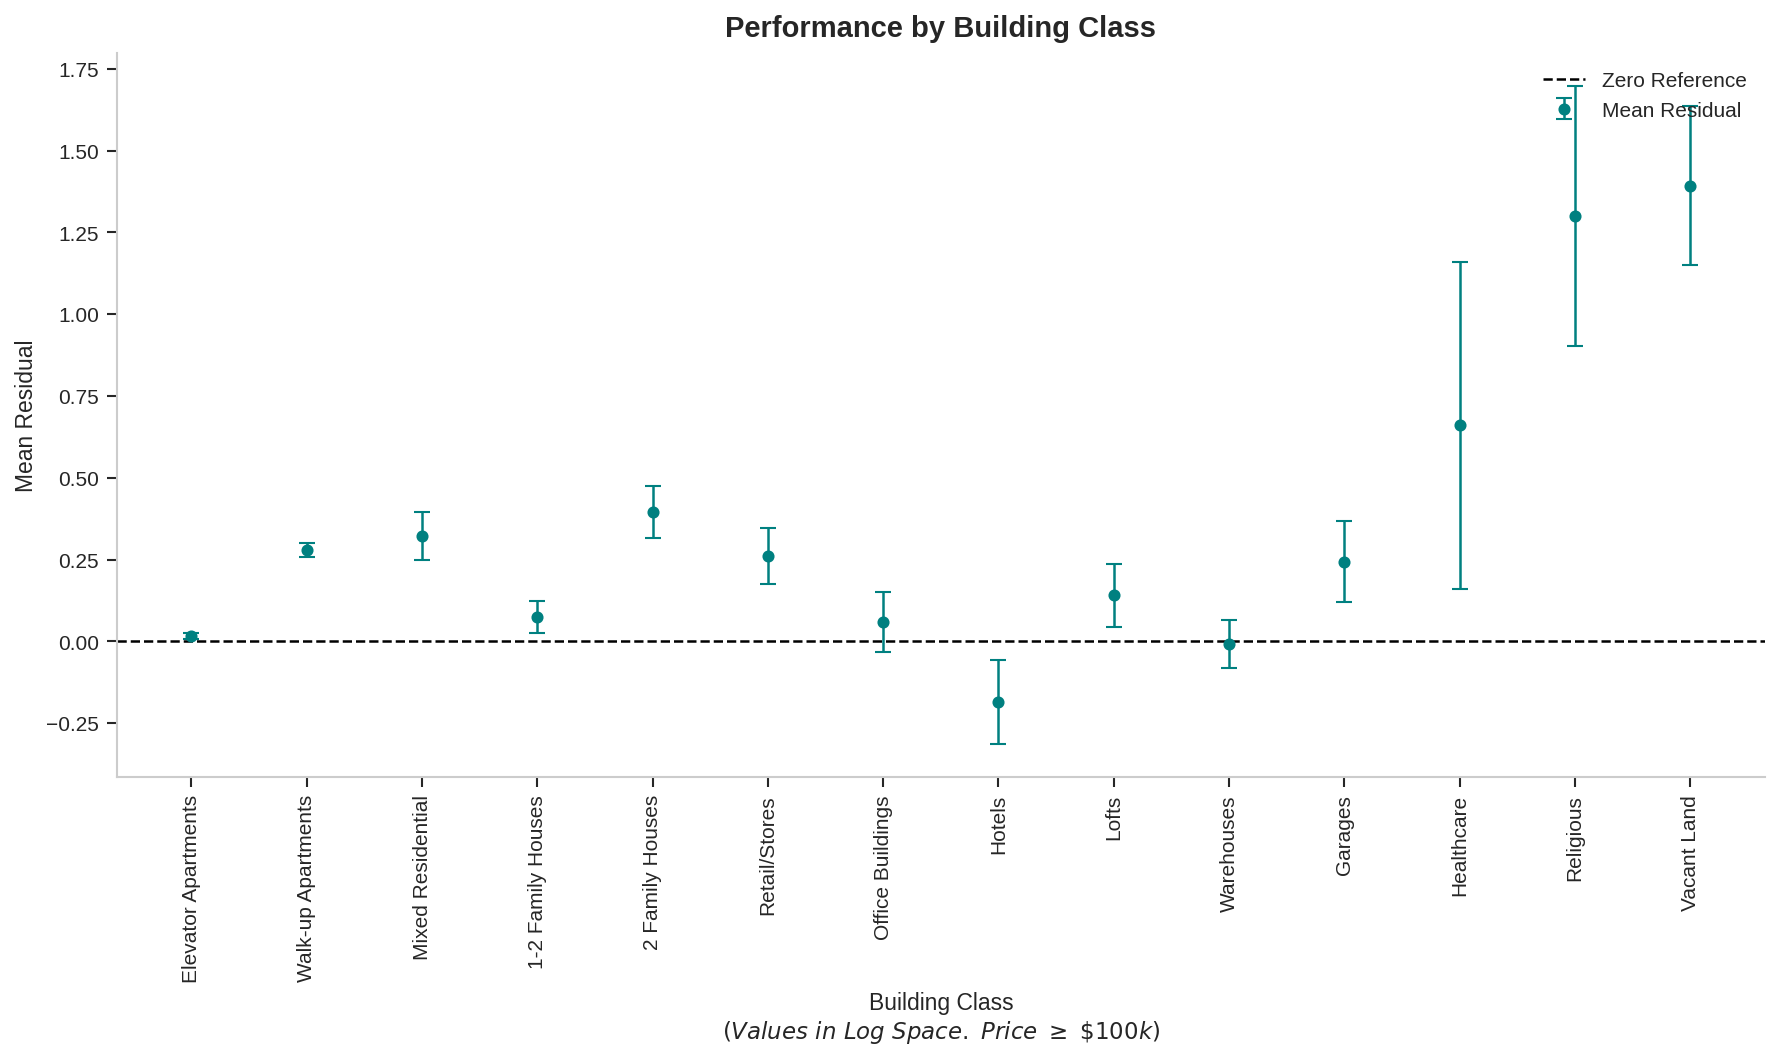
\includegraphics[width=0.7\textwidth]{residuals_by_bldg_class.png}
    \caption{Distribution of residuals broken down by Building Class. Commercial and mixed-use properties show significantly higher variance than single-family homes.}
    \label{fig:residuals-bldg}
\end{figure}

\begin{figure}[h]
    \centering
    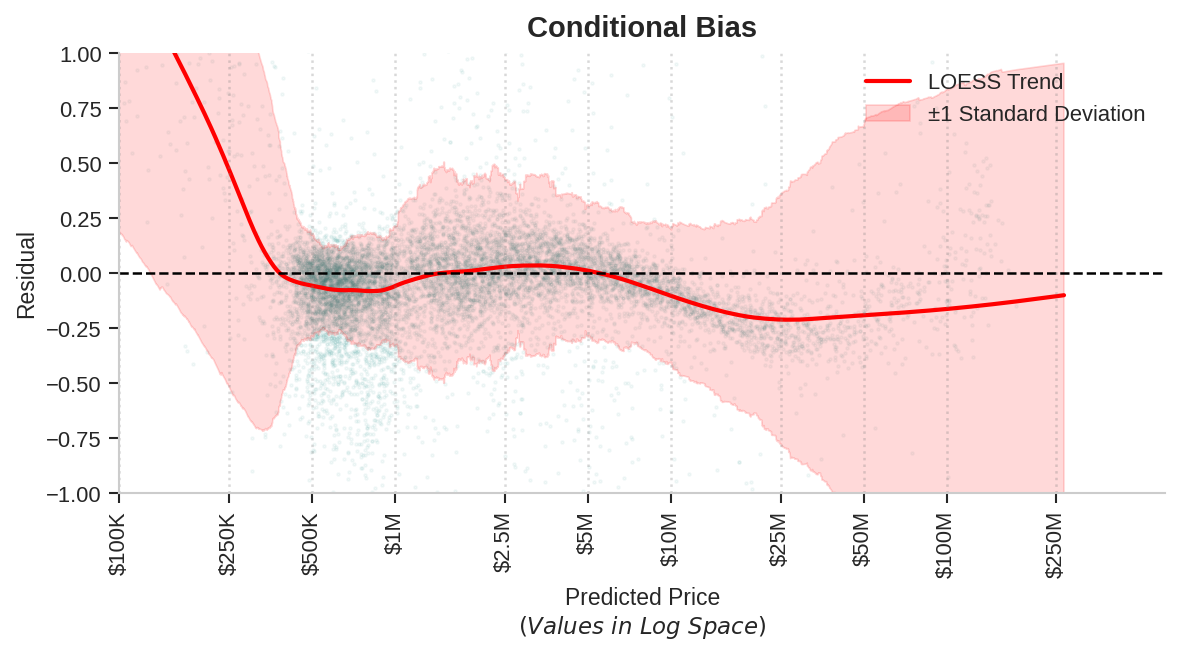
\includegraphics[width=0.48\textwidth]{residuals_vs_pred_bias.png}
    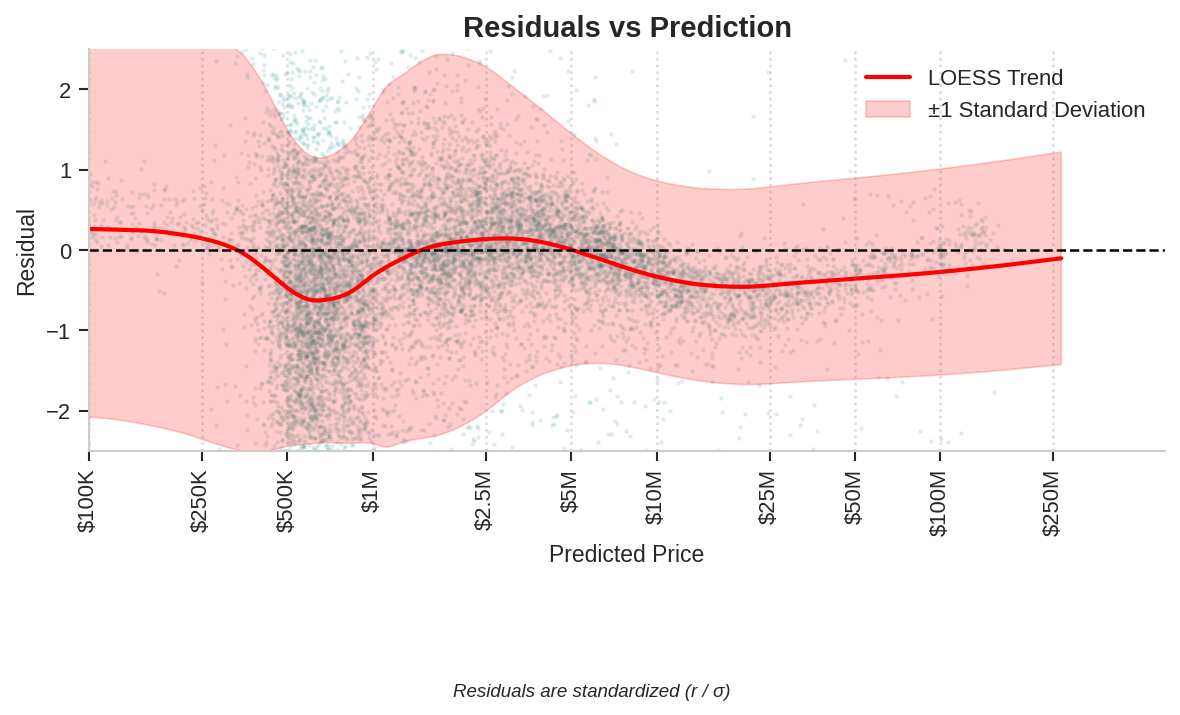
\includegraphics[width=0.48\textwidth]{residuals_standardized_vs_pred.png}
    \caption{Bias and Heteroscedasticity. Left: Raw residuals vs predicted (Bias check). Right: Standardized residuals ($z$-scores) vs predicted. The "fan" shape in the standardized plot explicitly visualizes heteroscedasticity.}
    \label{fig:residuals-bias-variance}
\end{figure}

To examine the deviations from the Gaussian likelihood assumption, we analyze the residuals in detail. The left panel of Figure~\ref{fig:residuals-log-appendix} compares the empirical histogram of log-price residuals against a fitted Normal distribution and a Student-$t$ distribution (with heavy tails). The clear heavy tails and peaked center (kurtosis $> 3$) confirm that a Gaussian likelihood is misspecified for this data, motivating the use of robust likelihoods in future work. The QQ plot in the right panel further visually quantifies this tail behavior, showing significant departures from the diagonal at extreme quantiles.

Figures~\ref{fig:residuals-bldg} and \ref{fig:residuals-bias-variance} break down performance by property type and price level. The boxplot by Building Class in Figure~\ref{fig:residuals-bldg} reveals heterogeneity in variance: commercial spaces strike broader ranges than uniform single-family homes. The scatter plots in Figure~\ref{fig:residuals-bias-variance} separate bias from variance. The raw residuals in the left panel show a flat trend, suggesting unbiasedness in expectation. However, the standardized residuals in the right panel reveal a distinct "fan" shape, indicating heteroscedasticity: uncertainty grows with the predicted price, a common feature in high-value real estate.

\section{Latent Space Density}

\begin{figure}[h]
    \centering
    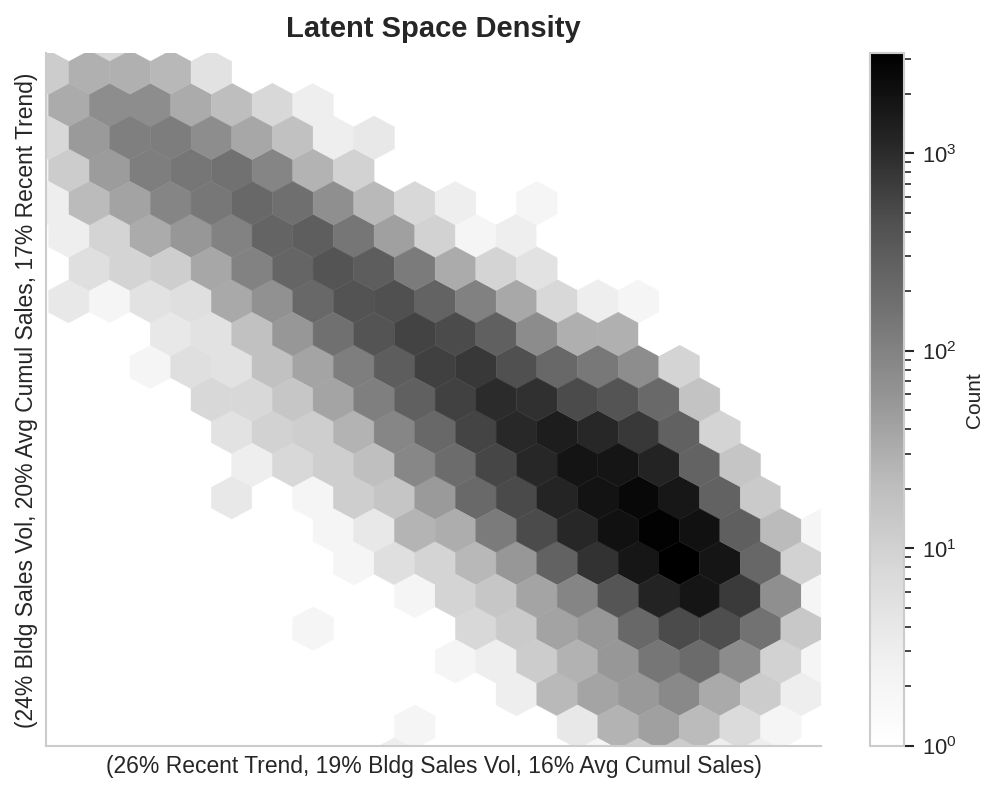
\includegraphics[width=0.48\textwidth]{latent_space_density.png}
    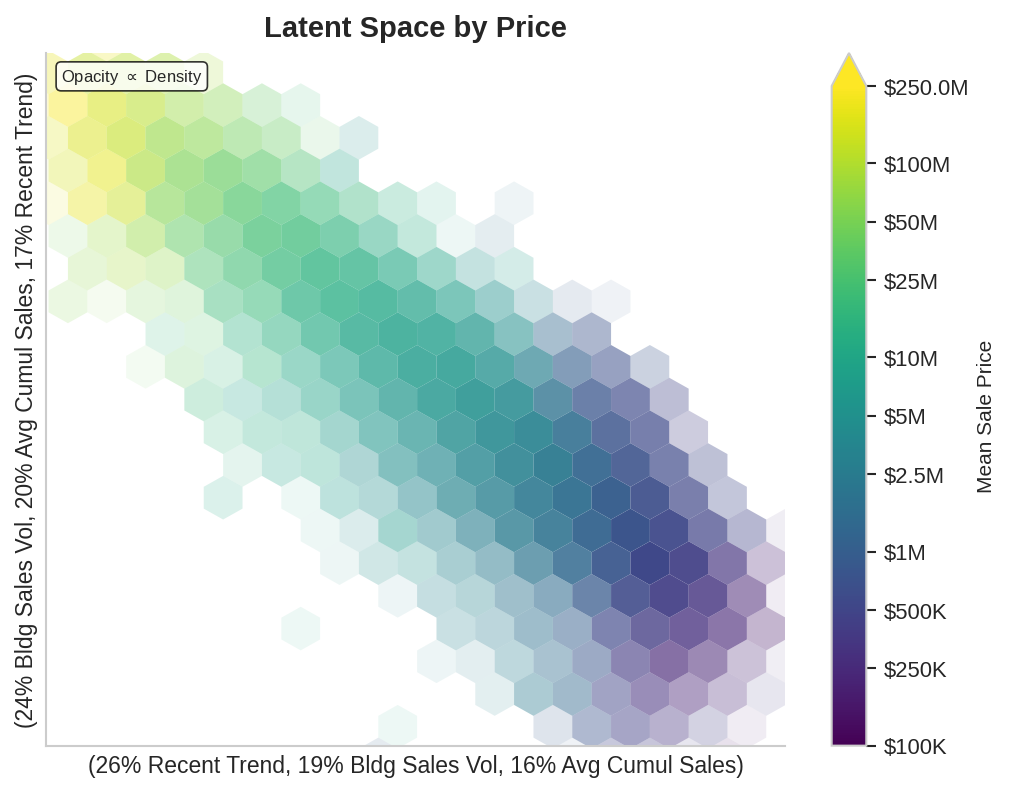
\includegraphics[width=0.48\textwidth]{latent_space_price_hexbin.png}
    \caption{Latent Space Manifold. Left: Density magnitude contours. Right: Mean log-sale price per hexbin, showing the valuations gradient.}
    \label{fig:latent-manifold}
\end{figure}

\begin{figure}[h]
    \centering
    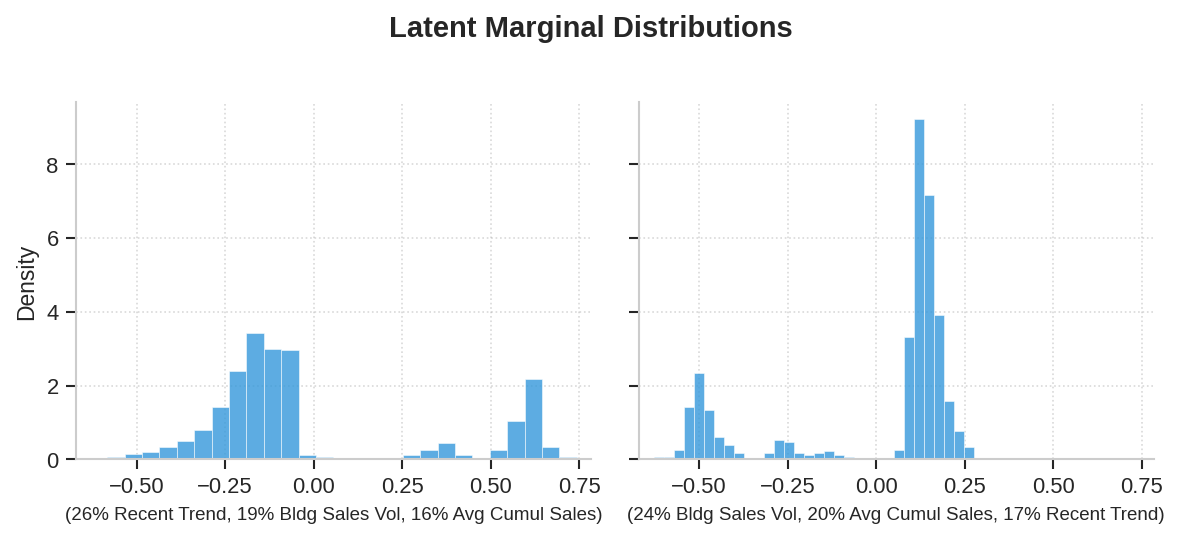
\includegraphics[width=0.8\textwidth]{latent_marginals.png}
    \caption{Marginal distributions of the latent dimensions, showing non-Gaussian peakedness.}
    \label{fig:latent-marginals}
\end{figure}

Figure~\ref{fig:latent-manifold} visualizes the aggregate posterior density. The contours in the left panel show that the learned representation $q(z)$ aggregates into a cohesive manifold. The hexbin plot on the right confirms that this manifold correlates smoothly with price. Additionally, Figure~\ref{fig:latent-marginals} shows the marginal distributions, confirming that while the aggregate posterior matches the prior support, it exhibits non-Gaussian peakedness characteristic of the Student-t prior.

\end{document}
